\documentclass{../sftex/sftex}

\usepackage{enumitem, mathtools, tikz}

\title{Raciocínio probabilístico --- redes Bayesianas}
\author{Emmanuel Podestá Jr., Gustavo Zambonin}
\email{\{emmanuel.podesta,gustavo.zambonin\}@grad.ufsc.br}
\src{https://github.com/zambonin/ufsc-ine5430}
\uniclass{Inteligência Artificial}
\classcode{UFSC-INE5430}

\usetikzlibrary{positioning}

\begin{document}

\maketitle

\centering
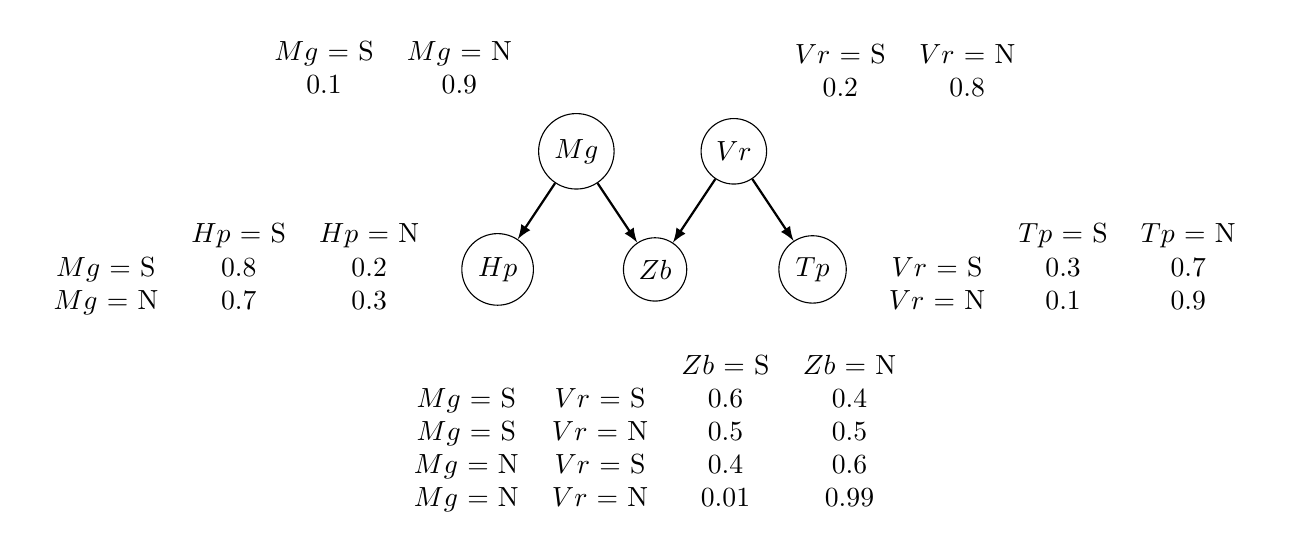
\begin{tikzpicture}
    \begin{scope}[every node/.style={circle, draw}]
        \node (Hp) at (0, 0)    {$Hp$};
        \node (Mg) at (1, 1.5)  {$Mg$};
        \node (Zb) at (2, 0)    {$Zb$};
        \node (Vr) at (3, 1.5)  {$Vr$};
        \node (Tp) at (4, 0)    {$Tp$};
    \end{scope}

    \begin{scope}[>=latex, thick]
        \draw[->] (Mg) -- (Hp);
        \draw[->] (Mg) -- (Zb);
        \draw[->] (Vr) -- (Zb);
        \draw[->] (Vr) -- (Tp);
    \end{scope}

    \begin{scope}[every node/.style={node distance=2mm}]
        \node[above left = of Mg] {
            \begin{tabular}{*{2}c}
                $Mg$ = S & $Mg$ = N \\
                0.1      & 0.9      \\
            \end{tabular}
        };

        \node[above right = of Vr] {
            \begin{tabular}{*{2}c}
                $Vr$ = S & $Vr$ = N \\
                0.2      & 0.8      \\
            \end{tabular}
        };

        \node[left = of Hp] {
            \begin{tabular}{*{3}c}
                         & $Hp$ = S & $Hp$ = N  \\
                $Mg$ = S & 0.8      & 0.2       \\
                $Mg$ = N & 0.7      & 0.3       \\
            \end{tabular}
        };

        \node[right = of Tp] {
            \begin{tabular}{*{3}c}
                         & $Tp$ = S & $Tp$ = N  \\
                $Vr$ = S & 0.3      & 0.7       \\
                $Vr$ = N & 0.1      & 0.9       \\
            \end{tabular}
        };

        \node[below = 5mm of Zb] {
            \begin{tabular}{*{4}c}
                         &          & $Zb$ = S & $Zb$ = N  \\
                $Mg$ = S & $Vr$ = S & 0.6      & 0.4       \\
                $Mg$ = S & $Vr$ = N & 0.5      & 0.5       \\
                $Mg$ = N & $Vr$ = S & 0.4      & 0.6       \\
                $Mg$ = N & $Vr$ = N & 0.01     & 0.99      \\
            \end{tabular}
        };
    \end{scope}
\end{tikzpicture}

\begin{enumerate}[label= (\textbf{\arabic*})]

    \item Observando a tabela para o nodo $Zb$:
        \begin{align*}
            P(Zb = N \mid Mg = N \land Vr = N) = \boldsymbol{0.99}
        \end{align*}

    \item Multiplica-se a probabilidade de todos os eventos serem verdadeiros
        entre si:
        \begin{align*}
            & P(Mg = S \land Vr = S \land Hp = S \land Zb = S \land Tp = S) \\
            & = P(Mg = S) \times P(Vr = S) \times P(Hp = S \mid Mg = S)
                \times P(Zb = S \mid Mg = S \land Vr = S)
                \times P(Tp = S \mid Vr = S) \\
            & = 0.1 \times 0.2 \times 0.8 \times 0.6 \times 0.3
                = \boldsymbol{0.00288}
        \end{align*}

    \item Multiplica-se a probabilidade dos nodos predecessores de $Zb$,
        quando este tem valor verdadeiro, e soma-se todos estes valores:
        \begin{align*}
            p_1 & = P(Mg = S \land Vr = S \land Zb = S)
                = 0.1 \times 0.2 \times 0.6 = 0.012 \\
            p_2 & = P(Mg = S \land Vr = N \land Zb = S)
                = 0.1 \times 0.8 \times 0.5 = 0.4 \\
            p_3 & = P(Mg = N \land Vr = S \land Zb = S)
                = 0.9 \times 0.2 \times 0.4 = 0.072 \\
            p_4 & = P(Mg = N \land Vr = N \land Zb = S)
                = 0.9 \times 0.8 \times 0.01 = 0.0072 \\
            P(Zb = S) & = \sum_{i=1}^4 p_i
                = 0.012 + 0.04 + 0.072 + 0.0072 = \boldsymbol{0.1312}
        \end{align*}

    \item Multiplica-se a probabilidade de $Vr$ e $Zb$ quando estes têm valor
        verdadeiro, aplicando também a probabilidade de $Mg$ nos dois casos,
        e soma-se estes valores:
        \begin{align*}
            p_1 & = P(Mg = S \land Vr = S \land Zb = S) \times P(Mg = S)
                = 0.6 \times 0.1 = 0.06 \\
            p_2 & = P(Mg = N \land Vr = S \land Zb = S) \times P(Mg = N)
                = 0.4 \times 0.9 = 0.36 \\
            P(Zb = S \mid Vr = S) & = \sum_{i=1}^2 p_i
                = 0.06 + 0.36 = \boldsymbol{0.42}
        \end{align*}

    \item Primeiramente, é necessário descobrir a probabilidade de $Zb$ dado
        que $Mg$ pode ou não acontecer:
        \begin{align*}
            p_1 & = P(Mg = S \land Vr = S \land Zb = S) \times P(Vr = S)
                = 0.6 \times 0.2 = 0.12 \\
            p_2 & = P(Mg = S \land Vr = N \land Zb = S) \times P(Vr = N)
                = 0.5 \times 0.8 = 0.4 \\
            P(Zb = S \mid Mg = S) & = \sum_{i=1}^2 p_i
                = 0.12 + 0.4 = 0.52
        \end{align*}
        \begin{align*}
            p_1 & = P(Mg = N \land Vr = S \land Zb = S) \times P(Vr = S)
                = 0.4 \times 0.2 = 0.08 \\
            p_2 & = P(Mg = N \land Vr = N \land Zb = S) \times P(Vr = N)
                = 0.01 \times 0.8 = 0.008 \\
            P(Zb = S \mid Mg = N) & = \sum_{i=1}^2 p_i
                = 0.08 + 0.008 = 0.088
        \end{align*}

        Então, utilizando probabilidade condicional e resultados anteriores:
        \begin{align*}
            P(Hp = S \mid Zb = S) & =
                \frac{P(Hp = S \land Zb = S \land Mg = S)
                    + P(Hp = S \land Zb = S \land Mg = N)}{P(Zb = S)} \\
                & = \frac{P(Mg = S) \times P(Hp = S \mid Mg = S)
                    \times P(Zb = S \mid Mg = S)}{P(Zb = S)} \\
                & + \frac{P(Mg = N) \times P(Hp = S \mid Mg = N)
                    \times P(Zb = S \mid Mg = N)}{P(Zb = S)} \\
                & = \frac{0.1 \times 0.8 \times 0.52
                    + 0.9 \times 0.7 \times 0.088}{0.1312}
                    = \boldsymbol{0.739\overline{63414}}
        \end{align*}

    \item A probabilidade de $Hp$ ser verdadeiro precisa ser calculada:
        \begin{align*}
            P(Hp = S) & =
                P(Hp = S \mid Mg = S) \times P(Mg = S)
                + P(Hp = S \mid Mg = N) \times P(Mg = N) \\
            & = 0.8 \times 0.1 + 0.7 \times 0.9 = 0.71
        \end{align*}

        Então, pelo Teorema de Bayes:
        \begin{align*}
            P(Zb = S \mid Hp = S) & =
                \frac{P(Hp = S \mid Zb = S) \times P(Zb = S)}{P(Hp = S)}
                \approx \frac{0.74 \times 0.1312}{0.71}
                \approx \boldsymbol{0.1367}
        \end{align*}

    \item A probabilidade de $Tp$ ser verdadeiro precisa ser calculada:
        \begin{align*}
            P(Tp = S) & =
                P(Tp = S \mid Vr = S) \times P(Vr = S)
                + P(Tp = S \mid Vr = N) \times P(Vr = N) \\
            & = 0.3 \times 0.2 + 0.1 \times 0.8 = 0.14
        \end{align*}

        Então, utilizando probabilidade condicional e resultados anteriores:
        \begin{align*}
            p_1 & = \frac{P(Zb = S \land Tp = S \land Hp = S
                \land Mg = S \land Vr = S)}{P(Tp = S \land Hp = S)} \\
            & = \frac{P(Mg = S) \times P(Hp = S \mid Mg = S)
                \times P(Zb = S \mid Mg = S \land Vr = S)
                \times P(Vr = S) \times P(Tp = S \mid Vr = S)}{P(Hp = S)
                \times P(Tp = S)} \\
            & = \frac{0.1 \times 0.8 \times 0.6 \times 0.2
                \times 0.3}{0.71 \times 0.14} \approx 0.02897
        \end{align*}
        \begin{align*}
            p_2 & = \frac{P(Zb = S \land Tp = S \land Hp = S
                \land Mg = S \land Vr = N)}{P(Tp = S \land Hp = S)} \\
            & = \frac{P(Mg = S) \times P(Hp = S \mid Mg = S)
                \times P(Zb = S \mid Mg = S \land Vr = N)
                \times P(Vr = N) \times P(Tp = S \mid Vr = N)}{P(Hp = S)
                \times P(Tp = S)} \\
            & = \frac{0.1 \times 0.8 \times 0.5 \times 0.8
                \times 0.1}{0.71 \times 0.14} \approx 0.03219
        \end{align*}
        \begin{align*}
            p_3 & = \frac{P(Zb = S \land Tp = S \land Hp = S
                \land Mg = N \land Vr = S)}{P(Tp = S \land Hp = S)} \\
            & = \frac{P(Mg = N) \times P(Hp = S \mid Mg = N)
                \times P(Zb = S \mid Mg = N \land Vr = S)
                \times P(Vr = S) \times P(Tp = S \mid Vr = S)}{P(Hp = S)
                \times P(Tp = S)} \\
            & = \frac{0.9 \times 0.7 \times 0.4 \times 0.2
                \times 0.3}{0.71 \times 0.14} \approx 0.1521
        \end{align*}
        \begin{align*}
            p_4 & = \frac{P(Zb = S \land Tp = S \land Hp = S
                \land Mg = N \land Vr = N)}{P(Tp = S \land Hp = S)} \\
            & = \frac{P(Mg = N) \times P(Hp = S \mid Mg = N)
                \times P(Zb = S \mid Mg = N \land Vr = N)
                \times P(Vr = N) \times P(Tp = S \mid Vr = N)}{P(Hp = S)
                \times P(Tp = S)} \\
            & = \frac{0.9 \times 0.7 \times 0.01 \times 0.8
                \times 0.1}{0.71 \times 0.14} \approx 0.00507
        \end{align*}
        \begin{align*}
            P(Zb = S \mid Tp = S \land Hp = S) & = \sum_{i=1}^4 p_i
            \approx 0.02897 + 0.03219 + 0.1521 + 0.00507
            \approx \boldsymbol{0.21833}
        \end{align*}

\end{enumerate}

\end{document}
